%%%%%%%%%%%%%%%%%%%%%%%%%%%%%%%%%%%%%%%%%%%%%%%%%%%%%%%%%%%%%%%%%%%%%%%%%%%%%%%%
\chapter{Placement Algorithms}
\label{ch:placement}
%%%%%%%%%%%%%%%%%%%%%%%%%%%%%%%%%%%%%%%%%%%%%%%%%%%%%%%%%%%%%%%%%%%%%%%%%%%%%%%%

The input for a placement algorithm consists of a geometry of spots
$\mathcal{S}$, the deposition sequence $N$, and a set of probes $\mathcal{P}$,
where each probe is assumed to have at least one embedding in $N$. The output is
a one-to-one assignment $\lambda$ of probes to spots. If there are more spots
than probes to place, one can add enough ``empty'' probes that do not introduce
any conflicts with the other probes (since light is never directed to their
spots).

All algorithms discussed in this section assume that an initial embedding of the
probes is given, which can be a left-most, right-most, synchronous or otherwise
pre-computed embedding --- a placement algorithm typically does not change the
given embeddings.

%%%%%%%%%%%%%%%%%%%%%%%%%%%%%%%%%%%%%%%%%%%%%%%%%%%%%%%%%%%%%%%%%%%%%%%%%%%%%%%%
\section{Optimal masks for uniform arrays}
\label{sec:placement_uniform}

\citet{Feldman1994} were the first to formally address the unintended
illumination problem. They showed how a placement for an \emph{uniform array}
with minimum number of border conflicts can be constructed using a
two-dimensional Gray code. Uniform arrays are arrays containing all $4^\ell$
probes of a given length $\ell$, which require a deposition sequence of length
$4\cdot \ell$. These arrays were initially developed for the technique known as
Sequencing by Hybridization (SBH).

\begin{figure}[t]\centering
\includegraphics[width=\textwidth]{place/uniform_placement}
\caption{\label{fig:uniform_placement}%
  Construction of a placement for uniform arrays (containing the complete set of
  $\ell$-mer probes) based on a two-dimensional Gray code, resulting in layouts
  with minimum number of border conflicts.}
\end{figure}

In general, the term Gray code refers to an ordering of a set of elements in
which successive elements differ in some pre-specified, usually small, way
\citep{Savage1997}. The construction of Feldman and Pevzner is based on a
two-dimensional Gray code compososed of string of length $\ell$ over a
four-letter alphabet. It generates an $2^\ell \times 2^\ell$ array filled with
$\ell$-mer probes in which each pair of adjacent probes (horizontally or
vertically) differs by exactly one letter. This construction is illustrated in
Fig.~\ref{fig:uniform_placement}. An $(\ell + 1)$-mer array is constructed by
first copying the $\ell$-mer array into the upper left quadrant of the
$(\ell + 1)$-mer array and reflecting it horizontally and vertically into the
other three quadrants. The letter in front of the probes in the upper left
quadrant of the $\ell$-mer array is added to all probes in the upper left
quadrant of the $(\ell + 1)$-mer array. The probes of the other three quadrants
are extended in the same way.

It can be shown that such placement generates masks with a minimum number of
border conflicts if the probes are synchronously embedded (see
Fig.~\ref{fig:uniform_masks}). However, because this construction is restricted
to uniform arrays and synchronous embeddings, it is of limited practical
importance for current microarrays.

\begin{figure}[t]
\begin{picture}(435,175)
\put(0,0){ \makebox(435,175){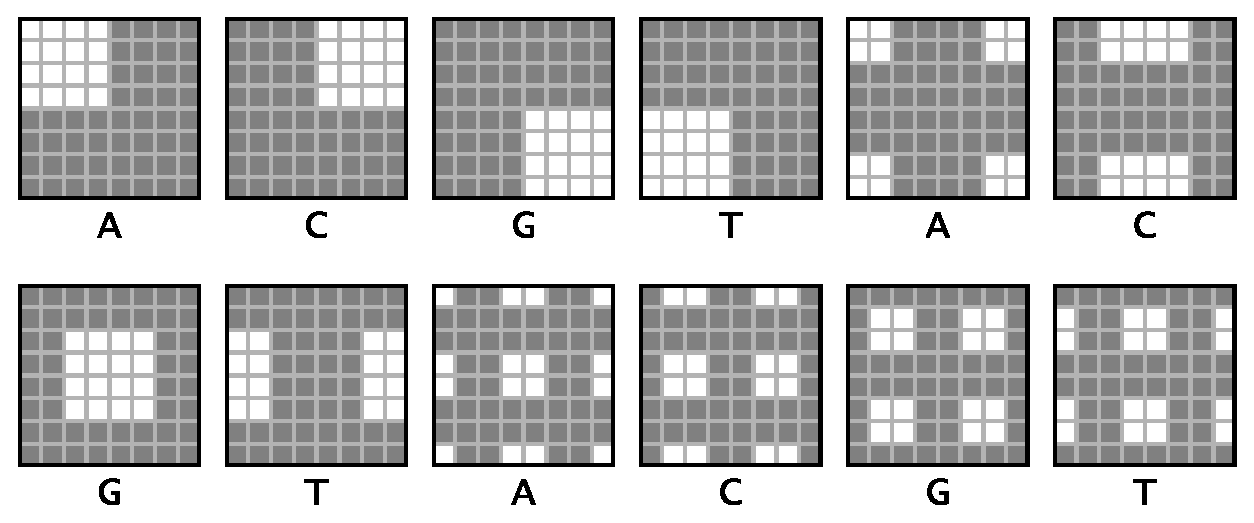
\includegraphics[width=\textwidth]{place/uniform_masks}}}
\end{picture}
\caption{\label{fig:uniform_masks}%
  Masks for the $8\times 8$ uniform array of Fig.~\ref{fig:uniform_placement}
  when probes are synchronously embedded into \{ACGT\}$^{3}$. Masked spots are
  represented by shaded squares, unmasked spots by white squares. Note that
  masks of the same cycle have the same number of border conflicts.}
\end{figure}

%%%%%%%%%%%%%%%%%%%%%%%%%%%%%%%%%%%%%%%%%%%%%%%%%%%%%%%%%%%%%%%%%%%%%%%%%%%%%%%%
\section{TSP and threading algorithms}
\label{sec:placement_threading}

The border length problem on arrays of arbitrary probes was first discussed by
\citet{Hannenhalli2002}. The article reports that the first Affymetrix chips
were designed using a heuristic for the traveling salesman problem (TSP). The
idea is to build a weighted graph with nodes representing probes, and edges
containing the Hamming distances between their embeddings (see
Eq.\ref{eq:hamming}). A TSP tour on this graph is heuristically constructed and
\emph{threaded} on the array in a row-by-row fashion
(Fig.~\ref{fig:threading}a).

For uniform arrays, every solution of the TSP corresponds to a (one-dimensional)
Gray code since consecutive elements in the tour differ in only one position,
thus minimizing border conflicts between consecutive probes. For general arrays,
a TSP solution also reduces border conflicts as consecutive probes in the tour
are likely to be similar. Threading the tour row-by-row leads to an arrangement
where consecutive probes in the same row have few border conflicts, but probes
in the same column may have very different embeddings.

Another problem of this approach is that the TSP is known to be NP-hard
\citep{Gross2004}, so computing an optimal TSP tour even for a small
$300\times 300$ array is not feasible, and only fast approximation algorithms
are suitable. In practice, Hannenhalli and co-workers managed to achieve
marginal improvements in tour cost using the 2-opt algorithm for TSP of
\citet{Lin1973} and an algorithm for weighted matching due to \citet{Gabow1976}.
Unfortunately, their efforts resulted in only $1.05\%$ reduction in tour cost
for a chip with $66\,000$ probes when compared to the greedy TSP algorithm
initially used at Affymetrix.

\begin{figure}[t]
\begin{picture}(435,130)
\put(-2,0){ \makebox(145,15){a)}}
\put(147,0){\makebox(145,15){b)}}
\put(292,0){\makebox(145,15){c)}}
\put(-2,15){ \makebox(145,115){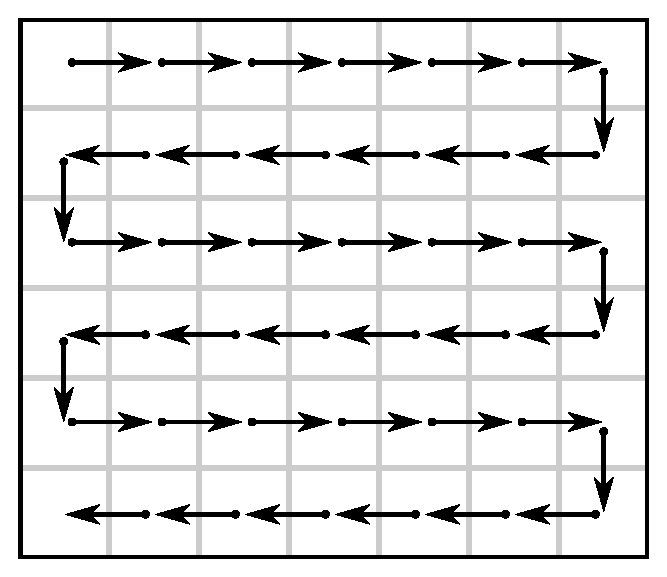
\includegraphics[width=0.3\textwidth]{0threading}}}
\put(147,15){\makebox(145,115){\includegraphics[width=0.3\textwidth]{1threading}}}
\put(292,15){\makebox(145,115){\includegraphics[width=0.3\textwidth]{2threading}}}
\end{picture}
\caption{\label{fig:threading}%
  Different ways of \emph{threading} probes on a chip. a) Standard row-by-row
  (0-threading); b) 1-threading; c) 2-threading.}
\end{figure}

Since improvements in the cost of the TSP tour seemed unlikely, Hannenhalli and
co-workers turned their attention to the threading of the tour on the chip. They
studied several threading alternatives, which they collectively called
\emph{$k$-threading} (Fig.~\ref{fig:threading}b,c).

A $k$-threading is a variation of the standard row-by-row threading, in which
the right-to-left and left-to-right paths are interspaced with alternating
upward and downward movements over $k$ sites (the row-by-row threading can be
seen as a $k$-threading with $k=0$); $k$ is called the \emph{amplitude} of the
threading. Hannenhalli and co-workers experimentally observed that 1-threading
may reduce total border length of layouts constructed with TSP tours in up to
20\% for large chips when compared to row-by-row threading.

%%%%%%%%%%%%%%%%%%%%%%%%%%%%%%%%%%%%%%%%%%%%%%%%%%%%%%%%%%%%%%%%%%%%%%%%%%%%%%%%
\section{Epitaxial placement}
\label{sec:placement_epitaxial}

A different strategy inspired by techniques used in the design of VLSI circuits,
called Epitaxial placement, was proposed by \citet{Kahng2002}. It essentially
grows a placement around a single starting ``seed'' using a greedy heuristic.
Although it was originally designed for chips with synchronous embeddings, it
can be trivially implemented for asynchronous embeddings as well.

The algorithm starts by placing a random probe in the center of the array and
continues to insert probes in spots adjacent to already-filled spots. Priority
is given to spots whose all four neighbors are full, in which case a probe with
the minimum number of border conflicts with the neighbors is placed. Otherwise,
all spots with $i \geq 1$ filled neighbors are examined. For each spot $s$, the
algorithm finds a non-assigned probe~$p$ whose number of border conflicts with
the filled neighbors of $s$, $c(s,p)$, is minimal, and assigns a normalized cost
$\bar{c}(s,p) := \sigma_i \cdot c(s,p) / i$ for this assignment, where
$0 < \sigma_i \leq 1$ are scaling coefficients (the authors propose
$\sigma_1 = 1$, $\sigma_2 = 0.8$, and $\sigma_3 = 0.6$). The assignment with
minimum $\bar{c}(s,p)$ is made and the procedure is repeated until all probes
have been placed.

In order to avoid repeated cost computations, the authors propose keeping a list
of probes candidates, for each spot, sorted by their normalized costs. This list
must be compiled at most four times, but on the average it is only computer two
times.

With this algorithm, Kahng and co-workers claim a further 10\% reduction in
border conflicts over TSP\,+\,1-threading. However, the Epitaxial algorithm have
at least quadratic time complexity as it examines every non-placed probe to fill
each spot, and large memory requirements if a list of probe candidates is kept
for each spot. Hence, like the TSP approach, it does not scale well to large
chips. In their experiments, the Epitaxial algorithm needed 274 seconds to
design a $100\times 100$ chip, but $4\,441$ seconds to design a $200\times 200$
chip, that is, a $16.2$-fold increase in running time for a 4-fold increase in
number of spots. Chips of larger dimensions could not be computed because of
prohibitively large running time and memory requirements.

%%%%%%%%%%%%%%%%%%%%%%%%%%%%%%%%%%%%%%%%%%%%%%%%%%%%%%%%%%%%%%%%%%%%%%%%%%%%%%%%
\section{Sliding-Window Matching}
\label{sec:placement_swm}

\begin{figure}[t!]
\centerline{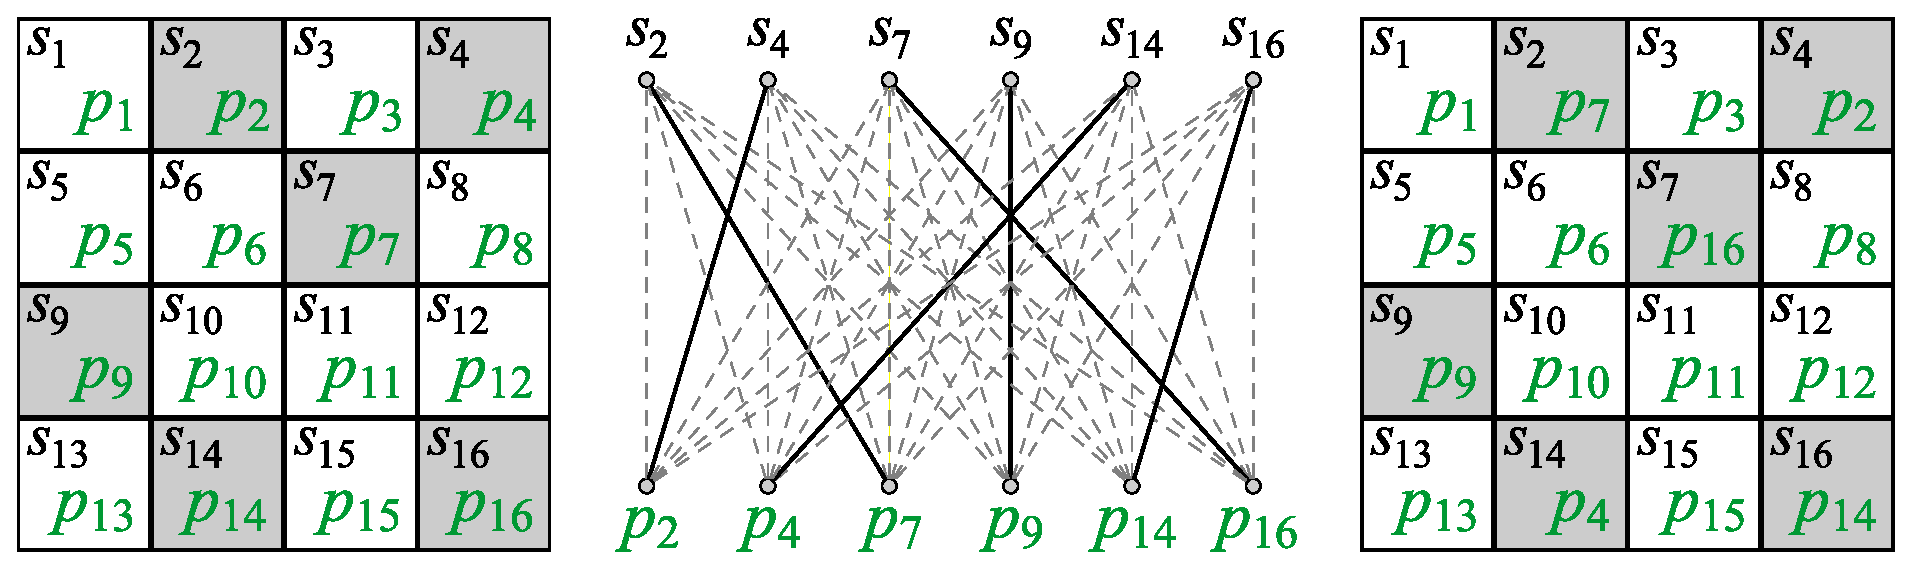
\includegraphics[width=\textwidth]{swm.eps}}
\begin{picture}(435,15)
\put(-2,0){ \makebox(145,15){a)}}
\put(147,0){\makebox(145,15){b)}}
\put(292,0){\makebox(145,15){c)}}
\end{picture}
\caption{\label{fig:swm}%
  Sliding-Window Matching algorithm. a) Initial arrangement of probes
  $p_1 \dots p_{16}$ inside a $4 \times 4$ window and the selected independent
  set of spots (shaded). b) Bipartite graph and a minimum weight perfect
  matching (dark edges). c) New arrangement inside the window according to the
  perfect matching.}%
\end{figure}

The Sliding-Window Matching algorithm \citep{Kahng2003}, SWM for short, is not
exactly a placement algorithm as it iteratively improves an existing placement
that can be constructed, for instance, by TSP\,+\,1-threading.

The authors noted that the TSP tour can be conveniently substituted by
lexicographically sorting the probe sequences or their binary embedding vectors
with a linear-time radix sort. The sorting is several times faster but it is
also likely to produce a worse initial placement than the TSP, with consecutive
embeddings being similar only in their first synthesis steps. The authors argue
that this is of little importance in practice given that this placement is only
used as a starting point for the SWM algorithm, and the lexicographical sorting
should be the choice for large microarrays because computing a TSP tour takes
prohibitively long for chips larger than $500\times 500$.

As its name implies, SWM works inside a window that starts at the top left of
the chip and slides from left to right, top to bottom, while maintaining a
certain amount of overlap between each iteration. When the window reaches the
right-end of the chip, it is re-started at the left-end of the next set of rows,
also retaining an overlap with the preceding set of rows.

At each iteration, the algorithm attempts to reduce the total border length
inside the window by relocating some of its probes (Fig.~\ref{fig:swm}a). First,
a random maximal independent set of spots is selected, and the probes assigned
to these spots are removed. The term independent refers to the fact that
selected spots can be re-assigned to probes without affecting the border length
of other selected spots. The algorithm then creates a bipartite graph with nodes
representing the removed probes and the now vacant spots (Fig.~\ref{fig:swm}b).
The edges of this graph are weighted with the number of border conflicts that
are generated by the corresponding assignment.  Finally, a minimum weight
perfect matching on this graph is computed, and the indicated assignments are
made (Fig.~\ref{fig:swm}c).

A minimum weight perfect matching requires polynomial time \citep{Gross2004},
but for the small graphs generated by SWM, it can be computed rather quickly.
The authors experimentally observed that the best results are obtained with
small window sizes (e.g. $6\times 6$) and an overlap of half the window size.
More over, employing less effort in each window and executing more cycles of
optimization is better than employing more effort in each window and executing
less cycles.

Selecting an independent set of spots ensures that the cost of each new
assignment can be computed independently of the other assignments. The SWM was
designed for border length minimization and it takes advantage of the fact that,
in this model, an independent set of spots can be constructed by selecting sites
that are not immediate neighbors (spots that do not share a common border). SWM
can be adapted for conflict index minimization (to our knowledge, this has not
been implemented yet) by using larger windows containing relatively sparse
independent sets. Therefore several random independent sets should be
constructed before moving the window.

%%%%%%%%%%%%%%%%%%%%%%%%%%%%%%%%%%%%%%%%%%%%%%%%%%%%%%%%%%%%%%%%%%%%%%%%%%%%%%%%
\section{Row-Epitaxial}
\label{sec:placement_reptx}

Row-Epitaxial \citep{Kahng2003} is a variant of the Epitaxial algorithm with two
main differences introduced to improve scalability: i) spots are filled in a
pre-defined order, namely, from top to bottom, left to right, and ii) only a
limited number $Q$ of probes candidates are considered for filling each spot.

Like SWM, Row-Epitaxial improves an initial placement that can be constructed
by, for example, Radix-sort\,+\,1-threading. For each spot $s$ with a probe $p$,
it looks at the next $Q$ probes that lie in close proximity (to the right or
below $s$), and swaps $p$ with the probe that generates the minimum number of
border conflicts between $s$ and its left and top neighbors.

In the experiments conducted by \citet{Kahng2003}, Row-Epitaxial was the best
large-scale placement algorithm (for border length minimization), achieving up
to 9\% reduction in border conflicts over the TSP\,+\,1-threading, whereas SWM
achieved slightly worse results but required significantly less time.

Row-Epitaxial can also be adapted to conflict index minimization by swapping a
probe of a spot $s$ with the probe candidate that minimizes the sum of conflict
indices in a region around $s$ restricted to those neighboring probes that are
to the left or above $s$ (those which have already found their final positions).

Table~\ref{tab:reptx} shows the results of using Row-Epitaxial for both border
length and conflict index minimization on chips with random probe sequences
(uniformly generated). Probes were lexicographically sorted and left-most
embedded into the standard 74-step Affymetrix deposition sequence and threaded
on the array with $k$-threading. The resulting layout was then used as a
starting point for Row-Epitaxial.

Although \citet{Hannenhalli2002} suggested that 1-threading is the best option
for laying out a TSP tour on the chip, our results show that increasing $k$
improves the initial layout produced by sorting\,+\,$k$-threading in terms of
border length and conflict index as well. However, the best initial layout does
not necessarily lead to the best final layout produced by Row-Epitaxial.

\begin{table}[p!]\centering
\caption{\label{tab:reptx}
  Normalized border length and average conflict index of layouts produced by
  Row-Epitaxial (Row-Eptx) on random chips of various dimensions, with initial
  layouts produced by Radix-sort\,+\,$k$-threading. Running times are reported
  in minutes and include the time for $k$-threading and Row-Epitaxial. All
  results are averages over a set of five chips.}
\footnotesize{
\begin{tabular*}{\hsize}{crrlrrrlrrr}
\vspace{1pt}
     &     &     & & \multicolumn{3}{c}{Border length minimization} & & \multicolumn{3}{c}{Conflict index minimization} \\ \cline{5-7} \cline{9-11}
\vspace{1pt}
Dim. & $Q$ & $k$ & & $k$-threading & Row-Eptx & Time                & & $k$-threading & Row-Eptx & Time \\
\hline
$300\times 300$ &  5K & 0 &  &      24.9649  & {\bf 18.2935} &   5.3 &  &      701.8698  &      462.5194  &  11.8 \\
                &     & 1 &  &      24.1235  &      18.2999  &   5.4 &  &      690.8091  & {\bf 462.4656} &  11.8 \\
                &     & 2 &  &      23.8695  &      18.3072  &   5.3 &  &      685.5916  &      462.6394  &  11.8 \\
                &     & 3 &  &      23.7993  &      18.3226  &   5.4 &  &      683.5980  &      462.5885  &  11.8 \\
                &     & 4 &  & {\bf 23.7588} &      18.3279  &   5.4 &  & {\bf 682.3542} &      462.7775  &  11.8 \\
\cline{2-11}
                & 10K & 0 &  &      24.9649  & {\bf 18.1477} &  10.5 &  &      701.8698  &      444.0354  &  22.2 \\
                &     & 1 &  &      24.1235  &      18.1529  &  10.5 &  &      690.8091  &      444.0904  &  22.4 \\
                &     & 2 &  &      23.8695  &      18.1519  &  10.5 &  &      685.5916  &      444.1960  &  22.2 \\
                &     & 3 &  &      23.7993  &      18.1591  &  10.5 &  &      683.5980  & {\bf 443.9850} &  22.3 \\
                &     & 4 &  & {\bf 23.7588} &      18.1603  &  10.5 &  & {\bf 682.3542} &      444.1745  &  22.2 \\
\cline{2-11}
                & 20K & 0 &  &      24.9649  &      18.0274  &  20.0 &  &      701.8698  &      426.7824  &  40.9 \\
                &     & 1 &  &      24.1235  &      18.0325  &  20.0 &  &      690.8091  &      426.8863  &  40.8 \\
                &     & 2 &  &      23.8695  &      18.0277  &  19.8 &  &      685.5916  &      426.8832  &  40.8 \\
                &     & 3 &  &      23.7993  & {\bf 18.0272} &  20.0 &  &      683.5980  &      426.8694  &  41.6 \\
                &     & 4 &  & {\bf 23.7588} &      18.0321  &  19.9 &  & {\bf 682.3542} & {\bf 426.6600} &  40.9 \\
\hline
$500\times 500$ &  5K & 0 &  &      24.2693  & {\bf 17.6000} &  15.6 &  &      693.5428  &      456.2042  &  33.5 \\
                &     & 1 &  &      23.3454  &      17.6095  &  15.4 &  &      682.2197  & {\bf 456.1167} &  33.5 \\
                &     & 2 &  &      23.0797  &      17.6246  &  15.5 &  &      676.4831  &      456.4575  &  33.5 \\
                &     & 3 &  &      22.9632  &      17.6474  &  15.3 &  &      672.8211  &      456.4878  &  33.7 \\
                &     & 4 &  & {\bf 22.9162} &      17.6670  &  15.5 &  & {\bf 671.2458} &      456.7849  &  33.4 \\
\cline{2-11}
                & 10K & 0 &  &      24.2693  & {\bf 17.4503} &  31.4 &  &      693.5286  &      438.6516  &  64.8 \\
                &     & 1 &  &      23.3454  &      17.4523  &  32.6 &  &      682.2197  &      438.6618  &  64.7 \\
                &     & 2 &  &      23.0797  &      17.4582  &  32.2 &  &      676.4831  & {\bf 438.5759} &  64.7 \\
                &     & 3 &  &      22.9632  &      17.4685  &  32.0 &  &      672.8211  &      438.7841  &  65.8 \\
                &     & 4 &  & {\bf 22.9162} &      17.4755  &  31.8 &  & {\bf 671.2458} &      438.9227  &  64.6 \\
\cline{2-11}
                & 20K & 0 &  &      24.2693  &      17.3303  &  63.7 &  &      693.5286  &      421.1773  & 125.1 \\
                &     & 1 &  &      23.3454  & {\bf 17.3297} &  65.5 &  &      682.2197  &      421.0770  & 125.5 \\
                &     & 2 &  &      23.0797  &      17.3308  &  66.6 &  &      676.4831  &      421.0952  & 126.0 \\
                &     & 3 &  &      22.9632  &      17.3344  &  66.1 &  &      672.8211  & {\bf 420.9112} & 123.7 \\
                &     & 4 &  & {\bf 22.9162} &      17.3376  &  64.8 &  & {\bf 671.2458} &      420.9534  & 124.4 \\
\hline
$800\times 800$ &  5K & 0 &  &      23.6818  & {\bf 16.9760} &  43.0 &  &      689.5915  & {\bf 447.9877} &  88.2 \\
                &     & 1 &  &      22.6092  &      16.9927  &  43.1 &  &      672.2191  &      448.0745  &  88.9 \\
                &     & 2 &  &      22.3205  &      17.0187  &  43.3 &  &      664.9477  &      448.6071  &  89.0 \\
                &     & 3 &  &      22.1958  &      17.0589  &  37.7 &  &      660.5476  &      448.9202  &  88.3 \\
                &     & 4 &  & {\bf 22.1279} &      17.1085  &  37.9 &  & {\bf 658.4852} &      449.1434  &  88.3 \\
\cline{2-11}
                & 10K & 0 &  &      23.6818  & {\bf 16.8032} &  95.0 &  &      689.5915  & {\bf 432.2326} & 179.6 \\
                &     & 1 &  &      22.6092  &      16.8111  &  95.7 &  &      672.2191  &      432.5542  & 179.3 \\
                &     & 2 &  &      22.3205  &      16.8235  &  95.2 &  &      664.9477  &      432.4991  & 178.1 \\
                &     & 3 &  &      22.1958  &      16.8353  &  84.6 &  &      660.5476  &      432.6598  & 179.2 \\
                &     & 4 &  & {\bf 22.1279} &      16.8622  &  83.7 &  & {\bf 658.4852} &      432.6423  & 178.9 \\
\cline{2-11}
                & 20K & 0 &  &      23.6818  & {\bf 16.6771} & 219.1 &  &      689.5915  & {\bf 415.6571} & 365.9 \\
                &     & 1 &  &      22.6092  &      16.6803  & 220.1 &  &      672.2191  &      415.7411  & 367.4 \\
                &     & 2 &  &      22.3205  &      16.6851  & 193.0 &  &      664.9477  &      415.6809  & 366.9 \\
                &     & 3 &  &      22.1958  &      16.6915  & 191.3 &  &      660.5476  &      415.7138  & 375.6 \\
                &     & 4 &  & {\bf 22.1279} &      16.7007  & 194.0 &  & {\bf 658.4852} &      415.7714  & 368.2 \\
\hline
\end{tabular*}}
\end{table}

Our results also confirm that the running time of Row-Epitaxial is $O(Qn)$,
i.e., linear in the chip size, where $Q$ is a user-defined parameter that
controls the number of probe candidades examined for each spot. In this way,
solution quality can be traded for running time: More candidates yield better
layouts but also demand more time.

%%%%%%%%%%%%%%%%%%%%%%%%%%%%%%%%%%%%%%%%%%%%%%%%%%%%%%%%%%%%%%%%%%%%%%%%%%%%%%%%
\section{Greedy}
\label{sec:placement_greedy}

As discussed in the previous section, the best results obtained with
Row-Epitaxial do necessarily come from the best initial layouts produced by
$k$-threading. This is probably because Row-Epitaxial does not take advantage of
the probe order used in $k$-threading when it looks for probe candidates for
filling a certain spot (Row-Epitaxial simply looks in the next $Q$ probes,
row-by-row, regardless of how the probes were threaded in the array).

In this section, we present a new placement algorithm, called Greedy, that
incorporates the Row-Epitaxial approach with a $k$-threading filling strategy.
Like Row-Epitaxial, spots are filled in a greedy fashion, i.e., for each spot
$s$, the algorithm examines $Q$ probe candidates and chooses the one that can be
placed at $s$ with minimum cost (Greedy can also be easily implemented for
border length as well as conflict index minimization). There are two main
differences, however. First, spots are filled with $k$-threading instead of
simply row-by-row.

Perhaps more importantly, Greedy sorts the probes lexicographically and keeps
them in a doubly-linked list, which is used to maintain the probe order during
the whole placement. Once a probe $p$ is selected to fill a certain spot, it is
removed from the list and the next search of candidades is performed around $p$
's former position, e.g., $Q/2$ probes to the left and to the right of $p$. In
this way, the algorithm always examines the probes that are more likely to be
similar to the last placed probe (which will be its neighbor on the chip).

Table~\ref{tab:greedy} shows the results of using Greedy for both border length
and conflict index minimization on the same set of (random) chips of
Table~\ref{tab:reptx}. Our results show that Greedy is slightly slower than
Row-Epitaxial (because it keeps the probe in a doubly-linked list) but
marginally better in terms of border length minimization and significantly
better in terms of conflict index minimization.

\begin{table}[p!]\centering
\caption{\label{tab:greedy}
  Normalized border length (NBL) and average conflict index (ACI) of layouts
  produced by Greedy on random chips of various dimensions. The results of
  Row-Epitaxial on the same set of chips (Table~\ref{tab:reptx}) is shown for
  comparison. Running times in minutes.}
\footnotesize{
\begin{tabular*}{\hsize}{crrrrrlrrrr}
\vspace{1pt}
     &         & \multicolumn{4}{c}{Border length minimization} & & \multicolumn{4}{c}{Conflict index minimization} \\ \cline{3-6} \cline{8-11}
\vspace{1pt}
     &         & \multicolumn{2}{c}{Row-Epitaxial} & \multicolumn{2}{c}{Greedy} & & \multicolumn{2}{c}{Row-Epitaxial} & \multicolumn{2}{c}{Greedy} \\
\vspace{1pt}
Dim. & $Q$ $k$ & NBL & Time & NBL & Time & & ACI & Time & ACI & Time \\
\hline
$300^2$         &  5K 0   &      24.9649  & 60.0 & {\bf 18.2935} &   5.3 &  &      701.8698  & 60.0 &      462.5194  &  11.8 \\
                &     1   &      24.1235  &      &      18.2999  &   5.4 &  &      690.8091  &      & {\bf 462.4656} &  11.8 \\
                &     2   &      23.8695  &      &      18.3072  &   5.3 &  &      685.5916  &      &      462.6394  &  11.8 \\
                &     3   &      23.7993  &      &      18.3226  &   5.4 &  &      683.5980  &      &      462.5885  &  11.8 \\
                &     4   & {\bf 23.7588} &      &      18.3279  &   5.4 &  & {\bf 682.3542} &      &      462.7775  &  11.8 \\
\cline{2-11}
                & 10K 0   &      24.9649  &      & {\bf 18.1477} &  10.5 &  &      701.8698  &      &      444.0354  &  22.2 \\
                &     1   &      24.1235  &      &      18.1529  &  10.5 &  &      690.8091  &      &      444.0904  &  22.4 \\
                &     2   &      23.8695  &      &      18.1519  &  10.5 &  &      685.5916  &      &      444.1960  &  22.2 \\
                &     3   &      23.7993  &      &      18.1591  &  10.5 &  &      683.5980  &      & {\bf 443.9850} &  22.3 \\
                &     4   & {\bf 23.7588} &      &      18.1603  &  10.5 &  & {\bf 682.3542} &      &      444.1745  &  22.2 \\
\cline{2-11}
                & 20K 0   &      24.9649  &      &      18.0274  &  20.0 &  &      701.8698  &      &      426.7824  &  40.9 \\
                &     1   &      24.1235  &      &      18.0325  &  20.0 &  &      690.8091  &      &      426.8863  &  40.8 \\
                &     2   &      23.8695  &      &      18.0277  &  19.8 &  &      685.5916  &      &      426.8832  &  40.8 \\
                &     3   &      23.7993  &      & {\bf 18.0272} &  20.0 &  &      683.5980  &      &      426.8694  &  41.6 \\
                &     4   & {\bf 23.7588} &      &      18.0321  &  19.9 &  & {\bf 682.3542} &      & {\bf 426.6600} &  40.9 \\
\hline
$500^2$         &  5K 0   &      24.2693  &      & {\bf 17.6000} &  15.6 &  &      693.5428  &      &      456.2042  &  33.5 \\
                &     1   &      23.3454  &      &      17.6095  &  15.4 &  &      682.2197  &      & {\bf 456.1167} &  33.5 \\
                &     2   &      23.0797  &      &      17.6246  &  15.5 &  &      676.4831  &      &      456.4575  &  33.5 \\
                &     3   &      22.9632  &      &      17.6474  &  15.3 &  &      672.8211  &      &      456.4878  &  33.7 \\
                &     4   & {\bf 22.9162} &      &      17.6670  &  15.5 &  & {\bf 671.2458} &      &      456.7849  &  33.4 \\
\cline{2-11}
                & 10K 0   &      24.2693  &      & {\bf 17.4503} &  31.4 &  &      693.5286  &      &      438.6516  &  64.8 \\
                &     1   &      23.3454  &      &      17.4523  &  32.6 &  &      682.2197  &      &      438.6618  &  64.7 \\
                &     2   &      23.0797  &      &      17.4582  &  32.2 &  &      676.4831  &      & {\bf 438.5759} &  64.7 \\
                &     3   &      22.9632  &      &      17.4685  &  32.0 &  &      672.8211  &      &      438.7841  &  65.8 \\
                &     4   & {\bf 22.9162} &      &      17.4755  &  31.8 &  & {\bf 671.2458} &      &      438.9227  &  64.6 \\
\cline{2-11}
                & 20K 0   &      24.2693  &      &      17.3303  &  63.7 &  &      693.5286  &      &      421.1773  & 125.1 \\
                &     1   &      23.3454  &      & {\bf 17.3297} &  65.5 &  &      682.2197  &      &      421.0770  & 125.5 \\
                &     2   &      23.0797  &      &      17.3308  &  66.6 &  &      676.4831  &      &      421.0952  & 126.0 \\
                &     3   &      22.9632  &      &      17.3344  &  66.1 &  &      672.8211  &      & {\bf 420.9112} & 123.7 \\
                &     4   & {\bf 22.9162} &      &      17.3376  &  64.8 &  & {\bf 671.2458} &      &      420.9534  & 124.4 \\
\hline
$800^2$         &  5K 0   &      23.6818  &      & {\bf 16.9760} &  43.0 &  &      689.5915  &      & {\bf 447.9877} &  88.2 \\
                &     1   &      22.6092  &      &      16.9927  &  43.1 &  &      672.2191  &      &      448.0745  &  88.9 \\
                &     2   &      22.3205  &      &      17.0187  &  43.3 &  &      664.9477  &      &      448.6071  &  89.0 \\
                &     3   &      22.1958  &      &      17.0589  &  37.7 &  &      660.5476  &      &      448.9202  &  88.3 \\
                &     4   & {\bf 22.1279} &      &      17.1085  &  37.9 &  & {\bf 658.4852} &      &      449.1434  &  88.3 \\
\cline{2-11}
                & 10K 0   &      23.6818  &      & {\bf 16.8032} &  95.0 &  &      689.5915  &      & {\bf 432.2326} & 179.6 \\
                &     1   &      22.6092  &      &      16.8111  &  95.7 &  &      672.2191  &      &      432.5542  & 179.3 \\
                &     2   &      22.3205  &      &      16.8235  &  95.2 &  &      664.9477  &      &      432.4991  & 178.1 \\
                &     3   &      22.1958  &      &      16.8353  &  84.6 &  &      660.5476  &      &      432.6598  & 179.2 \\
                &     4   & {\bf 22.1279} &      &      16.8622  &  83.7 &  & {\bf 658.4852} &      &      432.6423  & 178.9 \\
\cline{2-11}
                & 20K 0   &      23.6818  &      & {\bf 16.6771} & 219.1 &  &      689.5915  &      & {\bf 415.6571} & 365.9 \\
                &     1   &      22.6092  &      &      16.6803  & 220.1 &  &      672.2191  &      &      415.7411  & 367.4 \\
                &     2   &      22.3205  &      &      16.6851  & 193.0 &  &      664.9477  &      &      415.6809  & 366.9 \\
                &     3   &      22.1958  &      &      16.6915  & 191.3 &  &      660.5476  &      &      415.7138  & 375.6 \\
                &     4   & {\bf 22.1279} &      &      16.7007  & 194.0 &  & {\bf 658.4852} &      &      415.7714  & 368.2 \\
\hline
\end{tabular*}}
\end{table}

Talk about $k$-threading.

In terms of border length, we observed that increasing $Q$ above 5K has little
positive effect (see Fig.~\ref{fig:greedy_tradeoff}). For instance, on
$800\times 800$ chips, increasing $Q$ from 5K to 10K reduced the normalized
border length, on average, by only $0.66\%$ (from $17.1259$ to $17.0122$). In
terms of conflict index, increasing $Q$ even above 40K may result in significant
improvements for large chips. For instance, on $800\times 800$ chips, increasing
$Q$ from 40K to 80K reduced the average conflict index by $3.18\%$ (from
$381.8034$ to $369.6583$).

TODO: review figures above for border length.

The fact that increasing $Q$ has more effect in terms of conflict index is
probably because, in this measure, there is more room for optimization as the
conflicts can be moved to the extremities of the probes (while retaining the
same number of border conflicts) and a larger number of neighbors are involved.

\begin{figure}
%%
\begin{picture}(438,190)\footnotesize{
  \put(0,0){\makebox(219,200){
    %GNUPLOT: LaTeX picture with Postscript
    \begin{picture}(0,0)%
    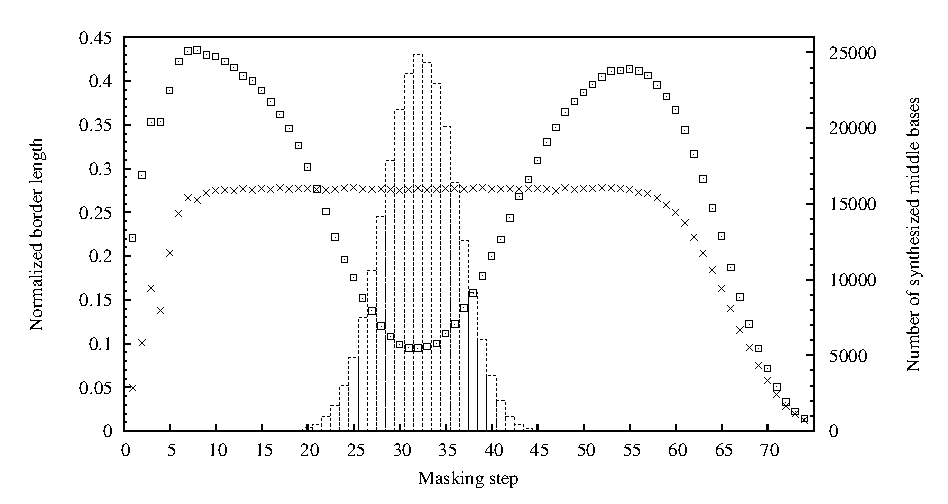
\includegraphics{place/tradeoff/bl}%
    \end{picture}%
    \begingroup
    \setlength{\unitlength}{0.0200bp}%
    \begin{picture}(11880,10044)(0,0)%
    \put(1750,1500){\makebox(0,0)[r]{\strut{} 16.6}}%
    \put(1750,2204){\makebox(0,0)[r]{\strut{} 16.8}}%
    \put(1750,2909){\makebox(0,0)[r]{\strut{} 17}}%
    \put(1750,3613){\makebox(0,0)[r]{\strut{} 17.2}}%
    \put(1750,4318){\makebox(0,0)[r]{\strut{} 17.4}}%
    \put(1750,5022){\makebox(0,0)[r]{\strut{} 17.6}}%
    \put(1750,5726){\makebox(0,0)[r]{\strut{} 17.8}}%
    \put(1750,6431){\makebox(0,0)[r]{\strut{} 18}}%
    \put(1750,7135){\makebox(0,0)[r]{\strut{} 18.2}}%
    \put(1750,7840){\makebox(0,0)[r]{\strut{} 18.4}}%
    \put(1750,8544){\makebox(0,0)[r]{\strut{} 18.6}}%
    \put(2000,1000){\makebox(0,0){\strut{} 4}}%
    \put(3018,1000){\makebox(0,0){\strut{} 8}}%
    \put(4037,1000){\makebox(0,0){\strut{} 16}}%
    \put(5055,1000){\makebox(0,0){\strut{} 32}}%
    \put(6073,1000){\makebox(0,0){\strut{} 64}}%
    \put(7092,1000){\makebox(0,0){\strut{} 128}}%
    \put(8110,1000){\makebox(0,0){\strut{} 256}}%
    \put(9128,1000){\makebox(0,0){\strut{} 512}}%
    \put(10147,1000){\makebox(0,0){\strut{} 1024}}%
    \put(6565,250){\makebox(0,0){\strut{}Time (min)}}%
    \put(6565,9294){\makebox(0,0){\strut{}Normalized border length}}%
    \end{picture}%
    \endgroup
  }}
  \put(220,0){\makebox(219,200){
    %GNUPLOT: LaTeX picture with Postscript
    \begin{picture}(0,0)%
    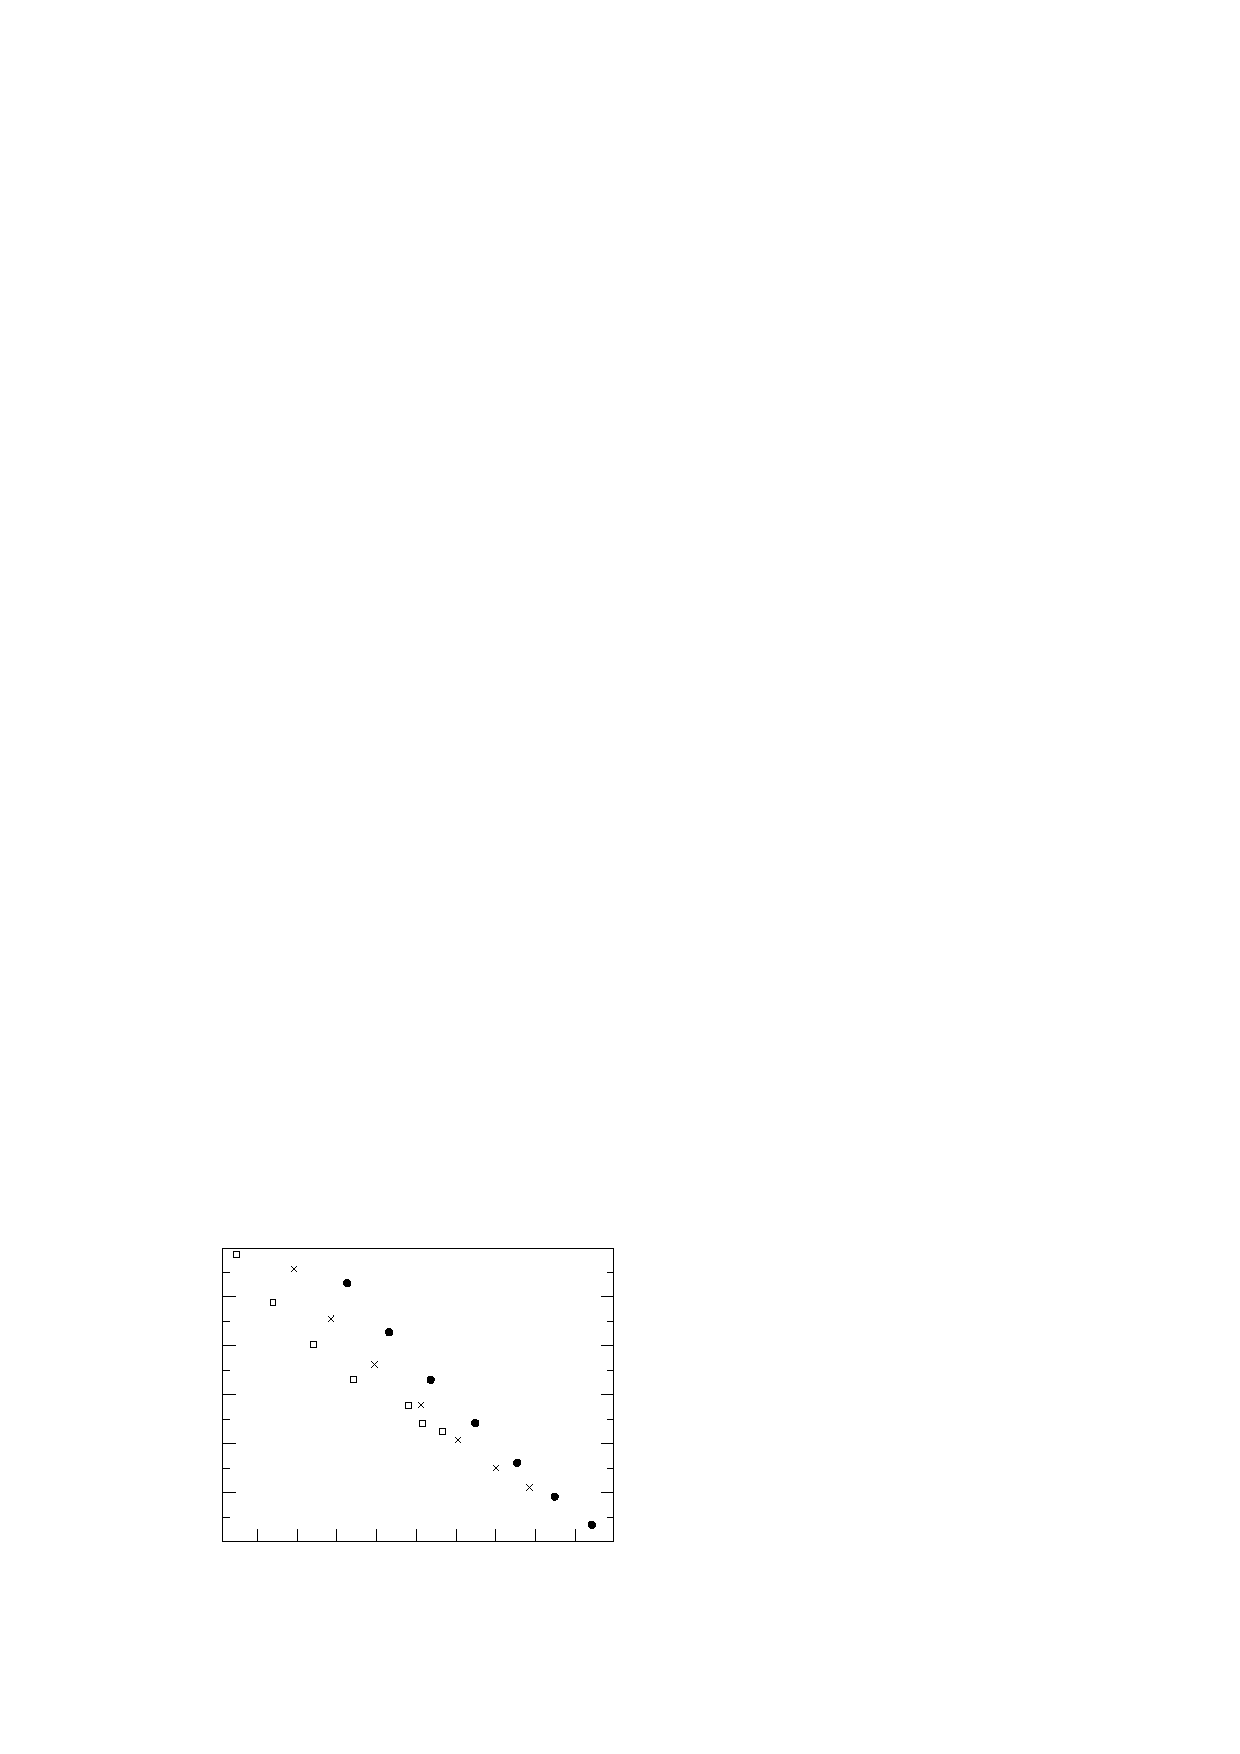
\includegraphics{place/tradeoff/ci}%
    \end{picture}%
    \begingroup
    \setlength{\unitlength}{0.0200bp}%
    \begin{picture}(11880,10044)(0,0)%
    \put(1500,1500){\makebox(0,0)[r]{\strut{} 360}}%
    \put(1500,2283){\makebox(0,0)[r]{\strut{} 370}}%
    \put(1500,3065){\makebox(0,0)[r]{\strut{} 380}}%
    \put(1500,3848){\makebox(0,0)[r]{\strut{} 390}}%
    \put(1500,4631){\makebox(0,0)[r]{\strut{} 400}}%
    \put(1500,5413){\makebox(0,0)[r]{\strut{} 410}}%
    \put(1500,6196){\makebox(0,0)[r]{\strut{} 420}}%
    \put(1500,6979){\makebox(0,0)[r]{\strut{} 430}}%
    \put(1500,7761){\makebox(0,0)[r]{\strut{} 440}}%
    \put(1500,8544){\makebox(0,0)[r]{\strut{} 450}}%
    \put(1750,1000){\makebox(0,0){\strut{} 4}}%
    \put(2796,1000){\makebox(0,0){\strut{} 8}}%
    \put(3842,1000){\makebox(0,0){\strut{} 16}}%
    \put(4889,1000){\makebox(0,0){\strut{} 32}}%
    \put(5935,1000){\makebox(0,0){\strut{} 64}}%
    \put(6981,1000){\makebox(0,0){\strut{} 128}}%
    \put(8027,1000){\makebox(0,0){\strut{} 256}}%
    \put(9073,1000){\makebox(0,0){\strut{} 512}}%
    \put(10120,1000){\makebox(0,0){\strut{} 1024}}%
    \put(6440,250){\makebox(0,0){\strut{}Time (min)}}%
    \put(6440,9294){\makebox(0,0){\strut{}Average conflict index}}%
    \end{picture}%
    \endgroup
  }}
}\end{picture}
%%
\caption{\label{fig:greedy_tradeoff}
  Trade-off between solution quality and running time with the Greedy algorithm
  on random chips of dimensions $300 \times 300$ ({\tiny $\Box$}),
  $500 \times 500$ ({\tiny $\times$}) and $800 \times 800$ ({\tiny $\bullet$}).
  The number $Q$ of candidates per spot are 5K, 10K, 20K, 40K, and 80K (from
  left to right. Layouts are measured by normalized border length (left) and
  average conflict index (right).}
\end{figure}
